% Permission is granted to copy, distribute and/or modify this document
% under the terms of the GNU Free Documentation License, Version 1.2
% or any later version published by the Free Software Foundation;
% with no Invariant Sections, no Front-Cover Texts, and no Back-Cover
% Texts.  A copy of the license is included in the section entitled "GNU
% Free Documentation License".
% Copyright 2015 EDF
%

%%%%%%%%%%%%%%%%%%%%%%%%%%%%%%%%%%%%%%%%%%%%%%%%%%%%%%%%%%%%%%%%%%%%%%%%%%%%%%%%%%%%%%%%%%
\section{Linear regression models}

Let us consider the general linear regression model:
\begin{equation}
\boxed{
Y \,=\, X \,\beta\, +\, \epsilon }
\end{equation}

Where $X$ is the design matrix of explanatory variables of size $(n \times p)$,
$Y$ is the vector of response values of size $(n)$,
$\beta$ is a vector of unknown parameters to be estimated of size $(p)$,
and $\epsilon $ is the error vector of size $(n)$; $\epsilon$ is assumed to follow the standard Normal distribution.\\


We define $G_X$ the Gram matrix of $X$ of size $(p\times p)$, $A_X$ its inverse,
and $H_X$ the projection matrix of size $(n\times n)$ by:
\begin{equation}
G_X \hat{=}X^T X  \quad,\quad  A_X \hat{=}(X^T X)^{-1}  \quad,\quad
H_X \hat{=} X_{}\,\big(X^T_{} \,X_{}\big)^{-1} \,X^T_{}  =  X_{}\,A_X \,X^T_{}
 \end{equation}

We define the \emph{Log likelihood} function by:
\begin{equation}
\log L(\beta,\sigma\mid Y)= -\frac{n}{2}\big(\log(2\pi)+ \log(\sigma^2)\big)- \frac{1}{2\sigma^2}\big(Y-X\beta\big)^T\,\big(Y-X\beta\big)
\end{equation}

The solution which maximizes the \emph{Log likelihood} function is:
\begin{equation}
\label{beta_sigma_opt}
  \hat{\beta} \,=\, \big(X^T_{} \,X_{}\big)^{-1} \,X^T \, Y
\quad,\quad
\hat{\sigma}^2 = \frac{1}{n}\big(Y-X \,\hat{\beta}\big)^T\,\big(Y-X \,\hat{\beta}\big)
\end{equation}
Using equation (\ref{beta_sigma_opt}), the maximum \emph{Log likelihood} turns into:
\begin{equation}
\label{maxLogLikelihood}
\log L(\hat{\beta},\hat{\sigma}\mid Y)=-\frac{n}{2}\big(\log(2\pi)+ \log(\hat{\sigma}^2)+1\big)
\quad \text{where} \quad
\hat{\sigma}^2 = \frac{1}{n}\big(Y-H_X\,Y\big)^T\,\big(Y-H_X\,Y \big)=\frac{1}{n}\|\,Y-H_X\,Y\,\|^2_2
\end{equation}

The residuals are defined by
\begin{equation}
\hat{\epsilon} = Y - H_X Y
\end{equation}

%%%%%%%%%%%%%%%%%%%%%%%%%%%%%%%%%%%%%%%%%%%%%%%%%%%%%%%%%%%%%%%%%%%%%%%%%%%%%%%%%%%%%%%%%%
\section{Architecture guide}

This section makes up the general specification design for the general linear model stepwise regression analysis
in OpenTURNS.

\subsection{LinearModel}

The \texttt{LinearModel} class is outdated and does not follow current best practices about metamodel classes.
We will introduce \texttt{LinearModelAlgorithm} and \texttt{LinearModelResult} classes.
All current uses of \texttt{LinearModel} have to be modified; it is used in classes \texttt{VisualTest},
\texttt{CorrelationAnalysis} and \texttt{LinearModelTest}. Class \texttt{LinearModelFactory} will be deprecated.

\begin{figure}[htb]
  \begin{center}
    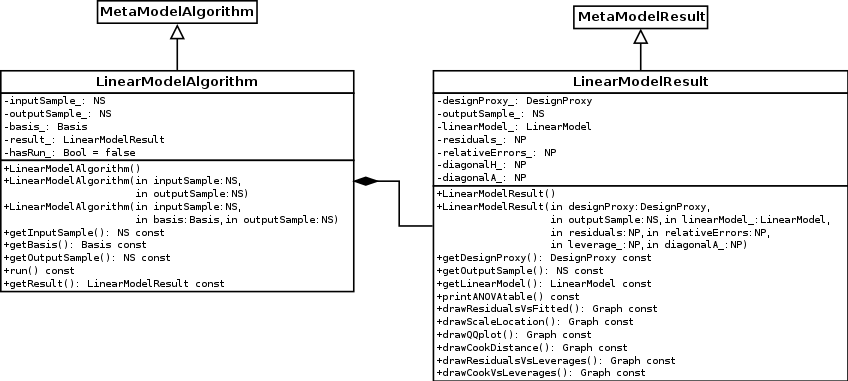
\includegraphics[scale=0.5]{LinearModelAlgorithm.png}
    \caption{LinearModelAlgorithm and LinearModelResult classes}\label{fig:archi:LinearModelAlgorithm}
  \end{center}
\end{figure}

\subsection{ANOVA table}

It is requested to give access to the following data:
\begin{itemize}
\item Linear model formula, in a textual form
\item Informations about residuals (minimum, maximum, median, mean, quantiles, standard deviation)
\item For each factor,
\begin{itemize}
\item its coefficient
\item its standard error
\item p-value for Student test
\item A visual symbol for significance test
\end{itemize}
\item Number of degrees of freedom
\item Coefficients $R^2$ and adjusted $R^2$
\item p-value of the Fisher test
\item normality tests on residuals (Kolmogorov-Smirnov, Anderson-Darling and $\chi^2$)
\end{itemize}

Note: Student test uses
\[
\frac{\hat{\beta}_i}{\sqrt{\frac{n}{n-p-1}\left[(X^T X)^{-1}\right]_{i,i}}}
\]

\subsection{Graphical diagnostics}

Several plots are provided by \texttt{LinearModelResult} class, see diagram class.
\begin{itemize}
\item \texttt{drawResidualsVsFitted} plots standardized residuals $\tilde{\epsilon}$ vs. fitted values, with
\[
\tilde{\epsilon}_i = \frac{\hat{\epsilon}_i}{\sqrt{\frac{n}{n-p-1}\hat{\sigma}^2 (1-H_{i,i})}}
\]
\item \texttt{drawQQPlot} plots $\sqrt{|\tilde{\epsilon}_i|}$ vs. theoretical quantiles.
\item \texttt{drawScaleLocation} plots $\sqrt{\tilde{\epsilon}_i}$ vs. fitted values.
\item \texttt{drawCookDistance} plots an histogram of Cook's distance
\[
D_i = \frac{\tilde{\epsilon}_i^2}{p} \left(\frac{H_{i,i}}{1-H_{i,i}}\right)
\]
\item \texttt{drawResidualsVsLeverages} plots standardized residuals $\tilde{\epsilon}$ vs leverages
\[
h_i = H_{i,i}
\]
Moreover, this plot also contains contour plot of function
\[
D(x,y) = \frac{y^2}{p}\left(\frac{x}{1-x}\right)
\]
for levels $0.5$ and $1$.
\item \texttt{drawCookVsLeverages} plots Cook's distance $\tilde{\epsilon}$ vs $\frac{h_i}{1-h_i}$.
\[
h_i = H_{i,i}
\]
Moreover, this plot also contains isolines of function
\[
\frac{py}{x}
\]
\end{itemize}

All these plots must display labels of some extremal points.  To this end, the following attributes
and methods will be added to \texttt{Cloud} and \texttt{BarPlot}:
\begin{verbatim}
   /** Setter for labels */
   Description getLabels() const;
   void setLabels(const Description & labels);
   /** Labels */
   Description labels_;
\end{verbatim}
The \texttt{labels} argument must have the same size as graph data, and only non-empty labels are
printed.

%%%%%%%%%%%%%%%%%%%%%%%%%%%%%%%%%%%%%%%%%%%%%%%%%%%%%%%%%%%%%%%%%%%%%%%%%%%%%%%%%%%%%%%%%%
\subsection{Stepwise regression methods}

The stepwise regression method consists in choosing the best predictive variables by an automatic procedure
 according to a selected model criterion ( Akaike information criterion (AIC), Bayesian information criterion (BIC)).
We define the sets of variables indices $ S_{min}\,\subseteq\, S_0\,\subseteq\, S_{max}$.
Let us consider $S$ a set of variables indices and $\# S$ the cardinal of $S$, the (AIC) and (BIC) criteria are:
\begin{itemize}
\item (AIC): $-2\,\log L(\hat{\beta},\hat{\sigma}\mid Y) + 2 \times \# S $
\item (BIC): $-2\,\log L(\hat{\beta},\hat{\sigma}\mid Y) + \log(n) \times \# S $ .
\end{itemize}

Using equation (\ref{maxLogLikelihood}) we get:
$(AIC) \,:\,  n\, \log(\hat{\sigma}^2) + C_1 + 2 \times \# S $ and $(BIC) \,:\,  n\, \log(\hat{\sigma}^2) + C_1 +\log(n) \times \# S $,
where the constant $C_1$ is defined by $ C_1 = n \big(\log(2\pi)+1\big)$. However for model comparisons, only differences in AIC (or BIC) criterion are meaningful, consequently the constant $C_1$ can be ignored,
which conveniently allows us to take as in R \texttt{step} method:
 \begin{eqnarray}
 AIC &:&  n\, \log(\hat{\sigma}^2) + 2 \times \# S  \\
 BIC &:&  n\, \log(\hat{\sigma}^2) +\log(n) \times \# S
\end{eqnarray}

There are three different algorithms: by using forward selection, backward selection, or both.

%%%%%%%%%%%%%%%%%%%%%%%%%%%%%%%%%%%%%%%%%%%%%%%%%%%%%%%%%%%%%%%%%%%%%%%%%%%%%%%%%%%%%%%%%%
\subsubsection{Forward selection}
This method starts with initial variables in the model (defined by the set of indices $S_0$), testing the addition of each variable
using a chosen model comparison criterion, adding the variable (if any) that improves the model the most, and repeating this process until none improves the model.
We define $X_{+i}$ the $(n \times (p+1))$ matrix composed by $X$ matrix and $x_i$ column: $X_{+i} = (X \,,\,x_i)$.
We define $\hat{\beta}_{+i}$ the vector of size $(p+1)$ and the scalar $\hat{\sigma}_{+i}^2$ by:
 \begin{equation}
  \hat{\beta}_{+i} \,=\, \big(X^T_{+i} \,X_{+i}\big)^{-1} \,X^T_{+i} \, Y
\quad,\quad
\hat{\sigma}_{+i}^2 = \frac{1}{n}\big(Y-X_{+i} \,\hat{\beta}_{+i}\big)^T\,\big(Y-X_{+i} \,\hat{\beta}_{+i}\big)
\end{equation}
We define $H_{+i} $ the $(n\times n)$ projection matrix by:
 \begin{equation}
\label{H+}
H_{+i}\, \,\hat{=} \, X_{+i}\,\big(X^T_{+i} \,X_{+i}\big)^{-1} \,X^T_{+i}
 \end{equation}
The Forward selection algorithm is listed on Algorithm~\ref{Forward_algo}.

%\IncMargin{3em}
\begin{algorithm}
\label{Forward_algo}
\KwData{ $S_0$, $S_{max}$,  \texttt{\color{black}{penalty\_}} = $\{2,\log(n)\}$,  \texttt{\color{black}{maxIter\_}} }
Initialization: $S^* = S_0$, $n_{iter} = 0 $\\
We compute $J^* = \log L(\hat{\beta},\hat{\sigma}\mid Y)$  \\
\While{ $n_{iter} <  \texttt{\color{black}{maxIter\_}} $  }{
 We compute $J^i = \log L(\hat{\beta}_{+i},\hat{\sigma}_{+i}\mid Y)$
where $\boxed{\,i = \displaystyle\arg \max_{j \in S_{max} \backslash S^*}\,\log L(\hat{\beta}_{+j},\hat{\sigma}_{+j}\mid Y) \,}  $\\
\uIf{$(J^i+$ \texttt{\color{black}{penalty\_}} $ < J^*) $ }{
$S^* =S^* \, \cup\,  i $\\
 $J^* = J^i$
}
\Else{
Quit
}
$n_{iter} = n_{iter} + 1$
}
\caption{Forward selection algorithm }
\end{algorithm}

Note that using equation (\ref{maxLogLikelihood}), we have:
 \begin{equation}
\arg   \displaystyle\max_{j \in S_{max} \backslash S^*}\,  \log L(\hat{\beta}_{+j},\hat{\sigma}_{+j}\mid Y) =
\arg \displaystyle\min_{j \in S_{max} \backslash S^*}\, \|\,Y-H_{+j}\,Y\,\|^2_2  \,\,
 \end{equation}
Consequently to find the best variable to add we can consider the least square of the residual term $:Y-H_{+i}\,Y$.



%%%%%%%%%%%%%%%%%%%%%%%%%%%%%%%%%%%%%%%%%%%%%%%%%%%%%%%%%%%%%%%%%%%%%%%%%%%%%%%%%%%%%%%%%%
\subsubsection{Backward selection}
This method starts with all candidate variables
(defined by the set of indices $S_{max}$), testing the deletion of each variable using a chosen model comparison criterion,
 deleting the variable (if any) that improves the model the most by being deleted, and repeating this process until no further improvement is possible.
We define $X_{-i}$ the $(n \times (p-1))$ matrix composed by $X$ matrix without the $x_i$ column.
We define $\hat{\beta}_{-i}$ the vector of size $(p-1)$ and the scalar $\hat{\sigma}_{-i}^2$ by:
 \begin{equation}
  \hat{\beta}_{-i} \,=\, \big(X^T_{-i} \,X_{-i}\big)^{-1} \,X^T_{-i} \, Y
\quad,\quad
\hat{\sigma}_{-i}^2 = \frac{1}{n}\big(Y-X_{-i} \,\hat{\beta}_{-i}\big)^T\,\big(Y-X_{-i} \,\hat{\beta}_{-i}\big)
\end{equation}
We define $H_{-i}$ the $(n\times n)$ projection matrix by:
 \begin{equation}
\label{H-}
H_{-i}\, \,\hat{=}\, X_{-i}\,\big(X^T_{-i} \,X_{-i}\big)^{-1} \,X^T_{-i}
 \end{equation}
The Backward selection algorithm is listed on Algorithm~\ref{Backward_algo}.
%\IncMargin{3em}
\begin{algorithm}
\label{Backward_algo}
\KwData{ $S_0$, $S_{min}$,  \texttt{\color{black}{penalty\_}} = $\{2,\log(n)\}$,  \texttt{\color{black}{maxIter\_}} }
Initialization: $S^* = S_0$, $n_{iter} = 0 $\\
We compute $J^* = \log L(\hat{\beta},\hat{\sigma}\mid Y)$  \\
\While{ $n_{iter} <  \texttt{\color{black}{maxIter\_}} $  }{
 We compute $J^i = \log L(\hat{\beta}_{-i},\hat{\sigma}_{-i}\mid Y)$
where $\boxed{\,i = \displaystyle\arg \max_{j \in S^*\backslash S_{min}}\,\log L(\hat{\beta}_{-j},\hat{\sigma}_{-j}\mid Y) \,}  $\\
\uIf{$(J^i-$ \texttt{\color{black}{penalty\_}} $ < J^*) $ }{
$S^* =S^* \, \backslash\,  i $\\
 $J^* = J^i$
}
\Else{
Quit
}
$n_{iter} = n_{iter} + 1$
}
\caption{Backward selection algorithm }
\end{algorithm}

Using equation (\ref{maxLogLikelihood}), we have:
 \begin{equation}
 \arg   \displaystyle\max_{j \in S^*\backslash S_{min}}\,  \log L(\hat{\beta}_{-j},\hat{\sigma}_{-j}\mid Y) =
\arg \displaystyle\min_{j \in S^*\backslash S_{min}}\, \|\,Y-H_{-j}\,Y\,\|^2_2  \,\,
 \end{equation}
Consequently to find the best variable to delete we can consider the least square of the residual term $:Y-H_{-i}\,Y$.

%%%%%%%%%%%%%%%%%%%%%%%%%%%%%%%%%%%%%%%%%%%%%%%%%%%%%%%%%%%%%%%%%%%%%%%%%%%%%%%%%%%%%%%%%%
\subsubsection{Bidirectional selection}

This method is a combination of the Forward and Backward selection. At each step, this method tests
the addition (Forward selection) and the deletion (Backward selection) of each variable using a chosen model comparison criterion,
select the method that improves the model the most, and repeat this process.

The Bidirectional selection algorithm (\ref{Bidirectional_algo}) is the following:
%\IncMargin{3em}
\begin{algorithm}
\label{Bidirectional_algo}
\KwData{ $S_0$, $S_{min}$, $S_{max}$,  \texttt{\color{black}{penalty\_}} = $\{2,\log(n)\}$,  \texttt{\color{black}{maxIter\_}} }
Initialization: $S^* = S_0$, $n_{iter} = 0 $\\
We compute $J^* = \log L(\hat{\beta},\hat{\sigma}\mid Y)$  \\
\While{ $n_{iter} <  \texttt{\color{black}{maxIter\_}} $  }{

 We compute $J^i = \log L(\hat{\beta}_{+i},\hat{\sigma}_{+i}\mid Y)$
where $\boxed{\,i = \displaystyle\arg \max_{j \in S_{max} \backslash S^*}\,\log L(\hat{\beta}_{+j},\hat{\sigma}_{+j}\mid Y) \,}  $\\

 We compute $J^{i'} = \log L(\hat{\beta}_{-i},\hat{\sigma}_{-i}\mid Y)$
where $\boxed{\,i' = \displaystyle\arg \max_{j \in S^*\backslash S_{min}}\,\log L(\hat{\beta}_{-j},\hat{\sigma}_{-j}\mid Y) \,}  $\\

\uIf{$(J^i+$ \texttt{\color{black}{penalty\_}} $ < J^*) $ {\bf or} $(J^{i'}-$ \texttt{\color{black}{penalty\_}} $< J^*)$}{
\uIf{$(J^i+$ \texttt{\color{black}{penalty\_}} $) <(J^{i'}-$\texttt{\color{black}{penalty\_}} $)$  }{
	$S^* =S^* \,\cup \,  i $\\
	$J^* = J^{i}$
}
\Else{
$S^* =S^* \,\backslash \,  i' $ \\
 $J^* = J^{i'}$
}
}
\Else{
Quit
}
$n_{iter} = n_{iter} + 1$
}
\caption{Bidirectional selection algorithm }
\end{algorithm}

Using equation (\ref{maxLogLikelihood}), we have:
 \begin{eqnarray}
 \arg   \displaystyle\max_{j \in S^*\backslash S_{min}}\,  \log L(\hat{\beta}_{-j},\hat{\sigma}_{-j}\mid Y) &=&
\arg \displaystyle\min_{j \in S^*\backslash S_{min}}\, \|\,Y-H_{-j}\,Y\,\|^2_2  \\
\arg   \displaystyle\max_{j \in S_{max} \backslash S^*}\,  \log L(\hat{\beta}_{+j},\hat{\sigma}_{+j}\mid Y)  &=&
\arg \displaystyle\min_{j \in S_{max} \backslash S^*}\, \|\,Y-H_{+j}\,Y\,\|^2_2
 \end{eqnarray}
 Consequently to find the best variable to add (resp. to delete), we can consider the least square of the residual term $:Y-H_{+i}\,Y$
 (resp.  $:Y-H_{-i}\,Y$).


\begin{figure}[htb]
  \begin{center}
    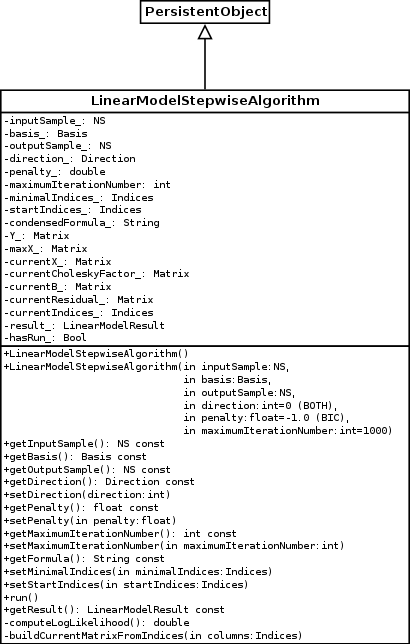
\includegraphics[scale=0.5]{LinearModelStepwiseAlgorithm.png}
    \caption{LinearModelStepwiseAlgorithm class}\label{fig:archi:LinearModelStepwiseAlgorithm}
  \end{center}
\end{figure}

%%%%%%%%%%%%%%%%%%%%%%%%%%%%%%%%%%%%%%%%%%%%%%%%%%%%%%%%%%%%%%%%%%%%%%%%%%%%%%%%%%%%%%%%%%
\section{Detailed implementation}
%%%%%%%%%%%%%%%%%%%%%%%%%%%%%%%%%%%%%%%%%%%%%%%%%%%%%%%%%%%%%%%%%%%%%%%%%%%%%%%%%%%%%%%%%%

Each selection method requires to find an index which minimizes some residual norm.
In this section, we explain how computations can be performed very efficiently, by
minimizing the number of operations.

\subsection{QR decomposition of matrix $X$}

Note that in practice $n >> p$ and consequently we don't want to compute $H_X$ the projection matrix of size $(n\times n)$.
We don't need to compute $A_X$ the inverse Gram matrix of $X$ of size $(p\times p)$ because we have to solve linear system, consequently
we use the QR decomposition of matrix $X$ into a product $X = Q_X\,R_X$ 
of an orthogonal matrix $Q_X$ of size $(n\times p)$ and an upper triangular matrix $R_X$ of size $(p\times p)$.\\

Using the QR decomposition of matrix $X$ we obtain :
  \begin{eqnarray}
  A_X &=& \big(X^T\,X\big)^{-1} = \big(R_X^T\,Q_X^T\,Q_X\,R_X\big)^{-1} = \big(R_X^T\,R_X\big)^{-1}= R_X^{-1}\,R_X^{-T} \\
  H_X &=& X\,\big(X^T\,X\big)^{-1}\,X^T  = X\,A_X\,X^T = Q_X\,R_X\,R_X^{-1}\,R_X^{-T}\,R_X^T\,Q_X^T =Q_X\, Q_X^T
 \end{eqnarray}
  

\subsection{Forward selection}

It can be shown that the inverse Gram matrix of $X_{+i}$ of size $((p+1)\times(p+1))$  can be represented by a block partition
\begin{equation}
\big(X^T_{+i} \,X_{+i}\big)^{-1} =
 \begin{bmatrix}
A_X + D_X\,D_X^T/C_X  & -D_X/C_X \\
D_X^T/C_X & 1/C_X
\end{bmatrix}
 \quad,\quad D_X = A_X\, X^T\,x_i
 \quad,\quad C_X = x_i^T x_i -x_i^T \,X\,A \, X^T\, x_i
 \end{equation}
Then the projection matrix $H_{+i}$ defined by equation (\ref{H+}) turns into:
 \begin{eqnarray}
H_{+i} & = &X\,A_X \, X^T + \frac{1}{C_X} \big(\,X\,A_X \, X^T\,x_i\,x_i^T\,X\,A_X \, X^T \,-\,X\,A_X \, X^T\,x_i\,x_i^T \,-\,x_i\,x_i^T \, X\,A_X \, X^T\,+\,x_i\,x_i^T \,\big)
\end{eqnarray}

We get the residual term:
 \begin{eqnarray}
Y-H_{+i}\,Y  & = & Y-X\,A_X \, X^T\,Y -\frac{(x_i^T\,X\,A_X \, X^T\,Y-x_i^T\,Y)}{C_X}\, \big(\,X\,A_X \, X^T\,x_i\, \,-\,x_i\,\big)\\
 & = & Y - H_X\,Y -\frac{x_i^T\,(Y\,-\,H_X\,Y)}{x_i^T\,(H_X\,x_i\, \,-\,x_i)}\, \big(\,H_X\,x_i\, \,-\,x_i\,\big)\\
\label{defH+Y}
 & = & Y - \hat{Y} -\frac{x_i^T\,(Y\,-\,\hat{Y})}{x_i^T\,(H_X\,x_i\, \,-\,x_i)}\, \big(\,H_X\,x_i\, \,-\,x_i\,\big)
\end{eqnarray}

\subsubsection{Implementation using QR decomposition:}


\begin{enumerate}
\item The vector $\hat{Y}=H_X\,Y=Q_X\,Q_X^T\,Y $ of size $(n)$ does not depend on the column $x_i$ to add.
The computation of this vector is done by two matrix-vector products. 
\item The vector $\,H_X\,x_i\,= Q_X\,Q_X^T\,x_i$ of size $(n)$ depends on the column $x_i$ to add.
The computation of this vector is done by two matrix-vector products. 
\end{enumerate}



\newpage
%%%%%%%%%%%%%%%%%%%%%%%%%%%%%%%%%%%%%%%%%%%%%%%%%%%%%%%%%%%%%%%%%%%%%%%%%%%%%%%%%%%%%%%%%%
\subsection{Backward selection}
The projection matrix $H_{-i}$ defined by equation (\ref{H-}) turns into:
 \begin{equation}
\label{H2-}
H_{-i}\, \,\hat{=}\, X_{-i}\,\big(X^T_{-i} \,X_{-i}\big)^{-1} \,X^T_{-i}
= X_{-i}\,A_{-i,-i} \, X^T_{-i} \,-\,\frac {1}{A_{i,i}}\,\big(X_{-i}\, A_{-i,i}\big)\, \big(X_{-i}\, A_{-i,i}\big)^T
 \end{equation}
where $A_{-i,-i}$ represents the matrix $A$ without row $i$ and column $i$,
$A_{-i,i}$ represents the column $i$ of the matrix $A$ without row $i$ and $A_{i,i}$ represents the diagonal term $i$ of the matrix $A$.\\

In order to avoid matrix copies, we want to use the matrix $A_X$ in the equation (\ref{H2-}) without creating matrices $A_{-i }$.
To this end, we define $X_{i=0}$ a matrix $X$ whose column $i$ contains only $0$, and $\forall B \in \mathbb{R}^p$ we note $\big[B\big]_{i=0}$ a copy of $B$ which has its $i$-th row equals to $0$.
We get: $\forall b \in \mathbb{R}^n\,,\, \forall c \in \mathbb{R}^p $
 \begin{equation}
\label{notation0}
X_{i=0}^T\,b \,=\,\big[X^T\,b\big]_{i=0} \quad,\quad X_{i=0}\,c \,=\,X\,\big[c\big]_{i=0}
 \end{equation}


 Using equation (\ref{notation0}), the projection matrix $H_{-i}$ defined by equation (\ref{H-}) turns into:
 \begin{eqnarray}
H_{-i}\, & = & X_{i=0}\,A_X\,X_{i=0}^T \,-\,\frac {1}{A_{i,i}}\,  \big(X_{i=0}\,A_{,i}\big) \big(X_{i=0}\,A_{,i}\big)^T   \\
& = & X_{i=0}\,A_X\,X_{i=0}^T \,-\,\frac {1}{A_{i,i}}\,  \big(X\,\big[A_{,i}\big]_{i=0}  \big) \big(X\,\big[A_{,i}\big]_{i=0} \big)^T
\end{eqnarray}
 Using equation (\ref{notation0}), we get the residual term:
 \begin{eqnarray}
Y-H_{-i}\,Y & = &Y- \,X_{i=0}\,A_X\,X_{i=0}^T\,Y \,+\,\frac {1}{A_{i,i}}\,  \big(X_{i=0}\,A_{,i}\,(A_{i,} X_{i=0}^T\,Y)\,\big)   \\
 & = & Y-\,X\,\big[\,A_X\,\big[X^T\,Y\big]_{i=0}\,\big]_{i=0} \,+\,\frac {1}{A_{i,i}}\,  \big( X\,\big[\,A_{,i}\,\big]_{i=0}\,\,(A_{i,} \,\big[X^T\,Y\big]_{i=0})\,\big)   \\
 & = & Y-\,X\,\big[\,A_X\,\big[X^T\,Y\big]_{i=0}\, -\,\frac {A_{i,} \,\big[X^T\,Y\big]_{i=0}}{A_{i,i}}\,A_{,i}\,      \big]_{i=0} \\
\label{defH-Y}
 & = & Y- \,X\,\big(\,A_X\,\big[X^T\,Y\big]_{i=0}\, -\,\frac {A_{i,} \,\big[X^T\,Y\big]_{i=0}}{A_{i,i}}\,A_{,i}\,\big)
\end{eqnarray}
Then we rewrite the residual term  equation (\ref{defH-Y}) using $e_i$ the vector of size $(p)$ with a $1$ in the $i^{th}$ coordinates and $0$ elsewhere.
We obtain :
 \begin{eqnarray}
Y-H_{-i}\,Y & = &Y- \,X\,\big(\,A_X\,(X^T\,Y-x_i^T\,Y\,e_i)\, -\,\frac {(A_X\,e_i)^T \,(X^T\,Y-x_i^T\,Y\,e_i)}{A_{i,i}}\,A_X\,e_i\,\big)  \\
 & = &  Y- \,X\, A_X\,X^T\,Y \,+\, (x_i^T\,Y)\,X\, A_X\,e_i \,+\,\frac { e_i^T\,A_X\,X^T\,Y-(x_i^T\,Y) \,e_i^T\,A_X\,e_i}{A_{i,i}} \,X\, A_X\,e_i  \\
 & = & Y- \hat{Y}  \,+\, (x_i^T\,Y)\,X\, A_X\,e_i \,+\,\frac { e_i^T\,A_X\,X^T\,Y}{A_{i,i}} \,X\, A_X\,e_i -(x_i^T\,Y)\,X\, A_X\,e_i \\
\label{defH-Y2}
 & = & Y- \hat{Y} \,+\,\,\frac { (X\, A_X\,e_i)^T\,Y}{A_{i,i}} \,X\, A_X\,e_i
\end{eqnarray}

\subsubsection{Implementation using QR decomposition:}

\begin{enumerate}
\item The vector $\hat{Y}=H_X\,Y=Q_X\,Q_X^T\,Y $ of size $(n)$ does not depend on the column $x_i$ to delete.
The computation of this vector is done by two matrix-vector products. 
\item The vector $\,X\, A_X\,e_i=Q_X\,R_X\,R_X^{-1}\,R_X^{-T}\,e_i = Q_X\,R_X^{-T}\,e_i $ of size $(n)$ depends on $x_i$ the column to delete.
The computation of this vector is done by two matrix-vector products :
\begin{enumerate}
\item First we compute the vector of size $(p)$: $b_i=R_X^{-T}\,e_i$.
\item Then we compute the vector of size $(p)$: $d_i=Q_X\,b_i$.
\end{enumerate}
\item The scalar $\,A_{i,i}=e_i^T\,A_X\,e_i =e_i^T\,R_X^{-1}\,R_X^{-T}\,e_i = (R_X^{-T}\,e_i)^T \,R_X^{-T}\,e_i$ depends on $x_i$ the column to delete.
The computation of this scalar is done by $\,A_{i,i}=b_i^T\,b_i$ .
\end{enumerate}


\newpage
%%%%%%%%%%%%%%%%%%%%%%%%%%%%%%%%%%%%%%%%%%%%%%%%%%%%%%%%%%%%%%%%%%%%%%%%%%%%%%%%%%%%%%%%%%
\subsection{Stepwise regression algorithms}
%\IncMargin{3em}
\begin{algorithm}
\KwData{ $S_{min}=$ \texttt{\color{blue}{minimalIndices}}, $S_0=$ \texttt{\color{blue}{startIndices}} , $S_{max}$  }
\BlankLine
Initialization: $S^* = S_0$ , $X = (x^k)_{k \in S^*}=\,$\texttt{\color{blue}{currentX\_}} , $Y=\,$\texttt{\color{blue}{Y\_}}  , $n_{iter} = 0 $ , $X_{max} =$ \texttt{\color{blue}{maxX\_}}  \\
\BlankLine
\While{ $n_{iter} < $  \texttt{\color{blue}{maxiter\_}}  }{
\BlankLine
We compute $J^* = \log L(\hat{\beta},\hat{\sigma}\mid Y)$ using  \texttt{\color{blue}{computeLogLikelihood()}}
which compute the Cholesky decomposition of the Gram matrix $G_X=X^T\,X$ : $L_X  \,/\, L_X\,L_X^T\,=\,G_X$.\\
Initialization: $J^i = +\infty$, $J^{i'} = +\infty$,  $ L_X=\,$\texttt{\color{blue}{currentCholeskyFactor\_}}, $B_X = X^T \,Y=\,$\texttt{\color{blue}{currentB\_}}\\
\BlankLine
\If{$($ \texttt{\color{blue}{direction\_}}   $\in \big\{$ FORWARD,BOTH $\big\})$}{
We compute the $(n)$ vector: $ Y-\hat{Y}= Y-X\,\big(L_X \, L_X^T\big)^{-1}\,X^T\,Y $ by solving two linear systems \\
$ [\,F_i\,,\,i\,] =$  \texttt{\color{blue}{computeUpdateForward}}$(S_{max} \backslash S^*,X,X_{max},L_X,Y-\hat{Y}) $\\
$ J^{i} = n\, \log(\frac{1}{n}F_{{i}})$
}
\If{$($ \texttt{\color{blue}{direction\_}}   $\in \big\{$ BACKWARD,BOTH $\big\})$}{
	$ [\,F_{i'}\,,\,{i'}\,] =$ \texttt{\color{blue}{computeUpdateBackward}}$(S^*\backslash S_{min},X,Y,L_X,B_X) $\\
	$ J^{i'} = n\, \log(\frac{1}{n}F_{{i'}})$
}
\uIf{$(J^i+$ \texttt{\color{blue}{penalty\_}} $ < J^*) $ {\bf or} $(J^{i'}-$ \texttt{\color{blue}{penalty\_}} $< J^*)$}{
\uIf{$(J^i+$ \texttt{\color{blue}{penalty\_}} $) <(J^{i'}-$\texttt{\color{blue}{penalty\_}} $)$  }{
	$S^* =S^* \,\cup \,  i $
}
\Else{
$S^* =S^* \,\backslash \,  i' $
}
$X = (x^k)_{k \in S^*} $
}
\Else{
Quit
}
$n_{iter} = n_{iter} + 1$
}
We update $L_X=$\texttt{\color{blue}{currentCholeskyFactor\_}}, $B_X=$\texttt{\color{blue}{currentB\_}} using \texttt{\color{blue}{computeLogLikelihood()}} \\
We compute the $(p)$ vector: $\hat{\beta}= \big(L_X \, L_X^T\big)^{-1}\,B_X $ by solving two linear systems \\
We compute the $(n)$ vectors: $\hat{Y}=X\,\hat{\beta} \,, \,\hat{\varepsilon}=Y-\hat{Y}$
and the scalar $\hat{\sigma}^2 = \frac{1}{n} \,\hat{\varepsilon}^T\,\hat{\varepsilon}$  \\
We compute the scalar: $H_{i,i} = x_i^T\,\big(L_X \, L_X^T\big)^{-1}\,x_i$  by solving two linear systems \\
We construct \texttt{LinearModelResult} with parameters: $(X,Y,\hat{\varepsilon})$.
\caption{Stepwise method algorithm }
\end{algorithm}

\newpage
%%%%%%%%%%%%%%%%%%%%%%%%%%%%%%%%%%%%%%%%%%%%%%%%%%%%%%%%%%%%%%%%%%%%%%%%%%%%%%%%%%%%%%%%%%
\subsubsection{\texttt{ComputeUpdateForward} algorithm}

 The function \texttt{ComputeUpdateForward} compute the least square of the residual term $(Y-H_{+i}\,Y)$ using equation (\ref{defH+Y}).
 The \texttt{ComputeUpdateForward} algorithm (\ref{ComputeUpdateForward_algo}) is the following:

%\IncMargin{2em}
\begin{algorithm}
\label{ComputeUpdateForward_algo}
\SetKwInOut{Input}{Input}
\underline{\texttt{ComputeUpdateForward}}$(S_{max} \backslash S^*,X,X_{max},L_X,Y-\hat{Y})$\\
\Input{$(n \times p)$ matrix: \texttt{\color{blue}{X\_}} $\, =X\,$, $(n \times m)$ matrix: \texttt{\color{blue}{Xmax\_}}$\,= X_{max}\,$  }
\Input{$(n\times p)$ matrix: \texttt{\color{blue}{L\_}}$\,=L_X\,$, $(n)$ vector: \texttt{\color{blue}{epsilon\_}} $\,=Y-\hat{Y}\,$   }
\BlankLine
Initialisation: $F_i = +\infty$
\BlankLine
\For{($j \in S_{max} \backslash S^* $)}{
\BlankLine
We compute the $(n)$ vector: $d_{j}-x_j = X\,\big(L_X \, L_X^T\big)^{-1}\, X^T\,x_j -x_j $ by solving two linear systems \\
We compute the $(n)$ vector: $ Y-H_{+j}\,Y = Y-\hat{Y} -\frac{x_j^T\,(Y -\hat{Y})}{x_j^T\,(d_{j}-x_j )} \big(d_{j}-x_j \big)\,\, $\\
We compute the scalar: $F_j \hat{=}\|\,Y-H_{+j}\,Y\,\|^2_2 $\\
\If{$F_j \, < \, F_i $ }{
$F_i\,=\, F_j$ and $i=j$
}
}
\Return{ $F_i$ and $i$}
\caption{\texttt{ComputeUpdateForward} }
\end{algorithm}

%%%%%%%%%%%%%%%%%%%%%%%%%%%%%%%%%%%%%%%%%%%%%%%%%%%%%%%%%%%%%%%%%%%%%%%%%%%%%%%%%%%%%%%%%%
\subsubsection{\texttt{ComputeUpdateBackward} algorithm}

The function \texttt{ComputeUpdateBackward} compute the least square of the residual term  $(Y-H_{-i}\,Y)$ using equation (\ref{defH-Y}).
 The \texttt{ComputeUpdateBackward} algorithm (\ref{ComputeUpdateBackward_algo}) is the following:


%\IncMargin{2em}
\begin{algorithm}
\label{ComputeUpdateBackward_algo}
\SetKwInOut{Input}{Input}
\underline{\texttt{ComputeUpdateBackward}}$(S^*\backslash S_{min},X,Y,L_X,B_X)$\\
\Input{$(n \times p)$ matrix: \texttt{\color{blue}{X\_}} $\, =X\, $,  $(n)$ vector: \texttt{\color{blue}{Y\_}} $=Y\,$ }
\Input{$(p \times p)$ matrix: \texttt{\color{blue}{L\_}}  $\, =L_X\, $,$(p)$ vector: \texttt{\color{blue}{B\_}}$\, =B_X\,$  }
\BlankLine
Initialisation: $F_{i'} = +\infty$
\BlankLine
\For{($j \in  S^*\backslash S_{min}$)}{
\BlankLine
We compute the $(p)$ vector: $ d_{j} =\,\big(L_X \, L_X^T\big)^{-1}\,\big[B_X\big]_{j=0}$ by solving two linear systems\\
We compute the $(p)$ vector: $ a_{j} =\,\big(L_X \, L_X^T\big)^{-1}\,e_{j}$ by solving two linear systems\\
We compute the $(n)$ vector: $ Y- H_{-i}\,Y
\,=\,Y- \,X\,  \big(\,d_{j} \,-\,\frac {{(d_{j}})_j}{(a_{j})_j}\,a_{j}\,\big)\,\,  $\\
We compute the scalar: $F_j \hat{=}\|\,Y-H_{-}\,Y\,\|^2_2 $\\
\If{$F_j \, < \, F_{i'} $ }{
$F_{i'}\,=\, F_j$ and ${i'}=j$
}
}
\Return{ $F_{i'}$ and ${i'}$}
\caption{\texttt{ComputeUpdateBackward}}
\end{algorithm}
